\documentclass{article}
\usepackage[utf8]{inputenc}

\usepackage{xparse}
\usepackage{graphicx}
\usepackage[dutch]{babel}
\usepackage[dutch]{datetime}
\usepackage[style=numeric]{biblatex}
\usepackage{csquotes}
\usepackage{hyperref}
\usepackage{xcolor,colortbl}
\usepackage{minted}
\usepackage{import}
\usepackage[official]{eurosym}
\usepackage{subcaption}
\usepackage{pdfpages}
\usepackage{float}
\usepackage{tabularx}

\bibliography{references.bib}

% custom macros
\newcommand{\quotes}[1]{``#1''}

\hypersetup{
    colorlinks,
    citecolor=black,
    filecolor=black,
    linkcolor=black,
    urlcolor=black,
    linktoc=all
}

\title{IROB Documentatie}
\author{Joey de Ruiter \& Sergi Philipsen}
\date{\today}

\begin{document}

\maketitle

\vspace{10mm}

\centerline{
\includegraphics[height=100mm]{img/logo.png}}

\vspace{10mm}

\centerline{
    \textit{Hoe de \quotes{Tennis Ball Bot} tot stand is gekomen}
}
\centerline{
    \textit{Voor de minor: \quotes{Robotica, Domotica en Industriële automatisering} te Hogeschool Leiden}
}

\clearpage

\section*{Voorwoord}
\import{sections/}{chapters/foreword.tex}
\clearpage

% inhoudsopgave
\tableofcontents
\clearpage

\section{Inleiding}
\import{sections/}{chapters/preface.tex}
\clearpage

\section{Voor de sprint}
\import{sections/}{chapters/pre-sprint.tex}
\clearpage

\section{Sprint 1}
\import{sections/}{chapters/sprint-1.tex}
\clearpage

\section{Sprint 2}
\import{sections/}{chapters/sprint-2.tex}
\clearpage

\section{Reflectie}
\import{sections/}{chapters/reflection.tex}
\clearpage

\appendix
\import{sections/}{chapters/apendix.tex}
\section{Onderzoek}
\textit{Start vanaf de volgende pagina}
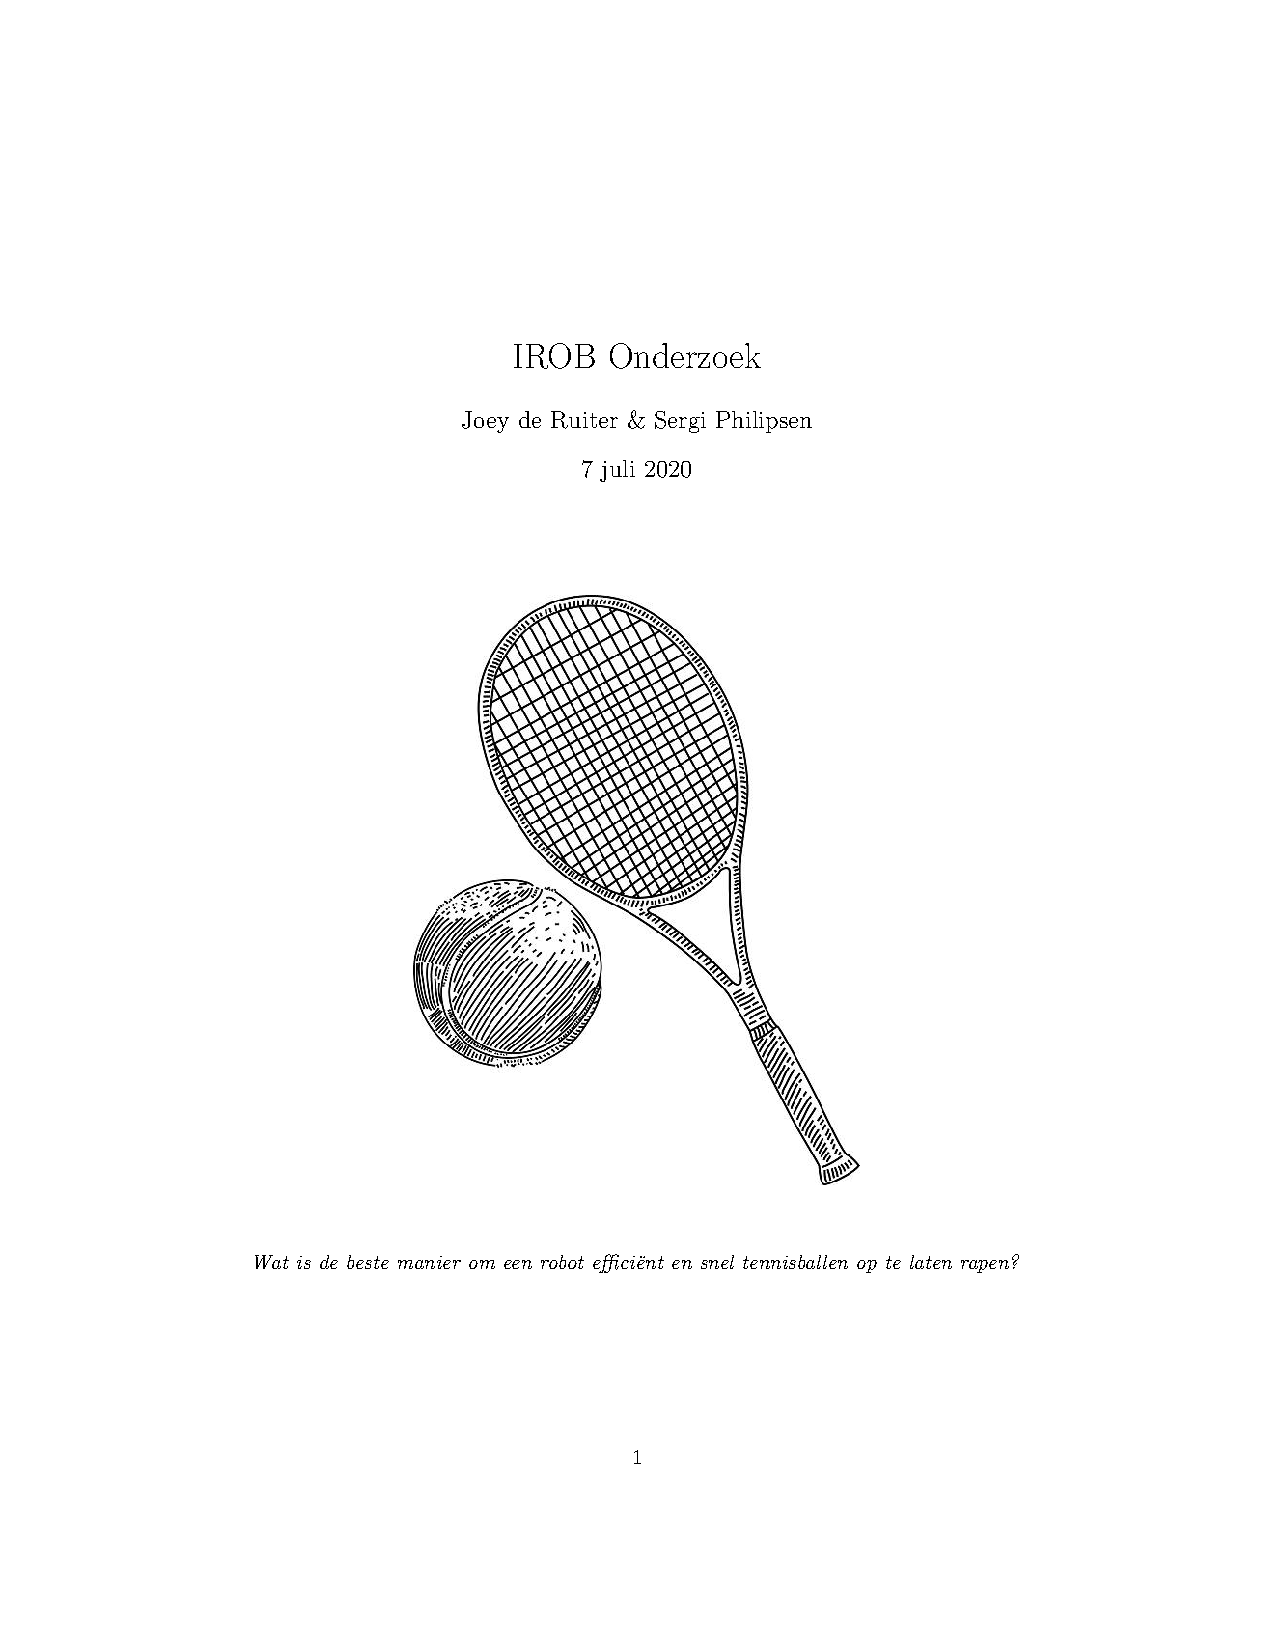
\includepdf[pages=-]{apendix/study.pdf}
\clearpage

\printbibliography[heading=bibintoc]
\clearpage

\end{document}